% !TeX TS-program = xelatex

\documentclass{resume}
\ResumeName{李宏扬}
% 如果想插入照片,请使用以下两个库。
\usepackage{graphicx}
\usepackage{tikz}

\begin{document}
\ResumeContacts{
  (+86)136-3436-6081,%
  \ResumeUrl{mailto:zjulihongyang@gmail.com}{zjulihongyang@gmail.com}%
}

% 如果想插入照片,请取消此代码的注释。
% 但是默认不推荐插入照片,因为这不是简历的重点。
% 如果默认的照片插入格式不能满足你的需求,你可以尝试调整照片的大小,或者使用其他的插入照片的方法。
% 不然,也可以先渲染 PDF 简历,然后用其他工具在 PDF 上叠加照片。
\begin{tikzpicture}[remember picture, overlay]
\node [anchor=north east, inner sep=1.5cm]  at (current page.north east) 
      {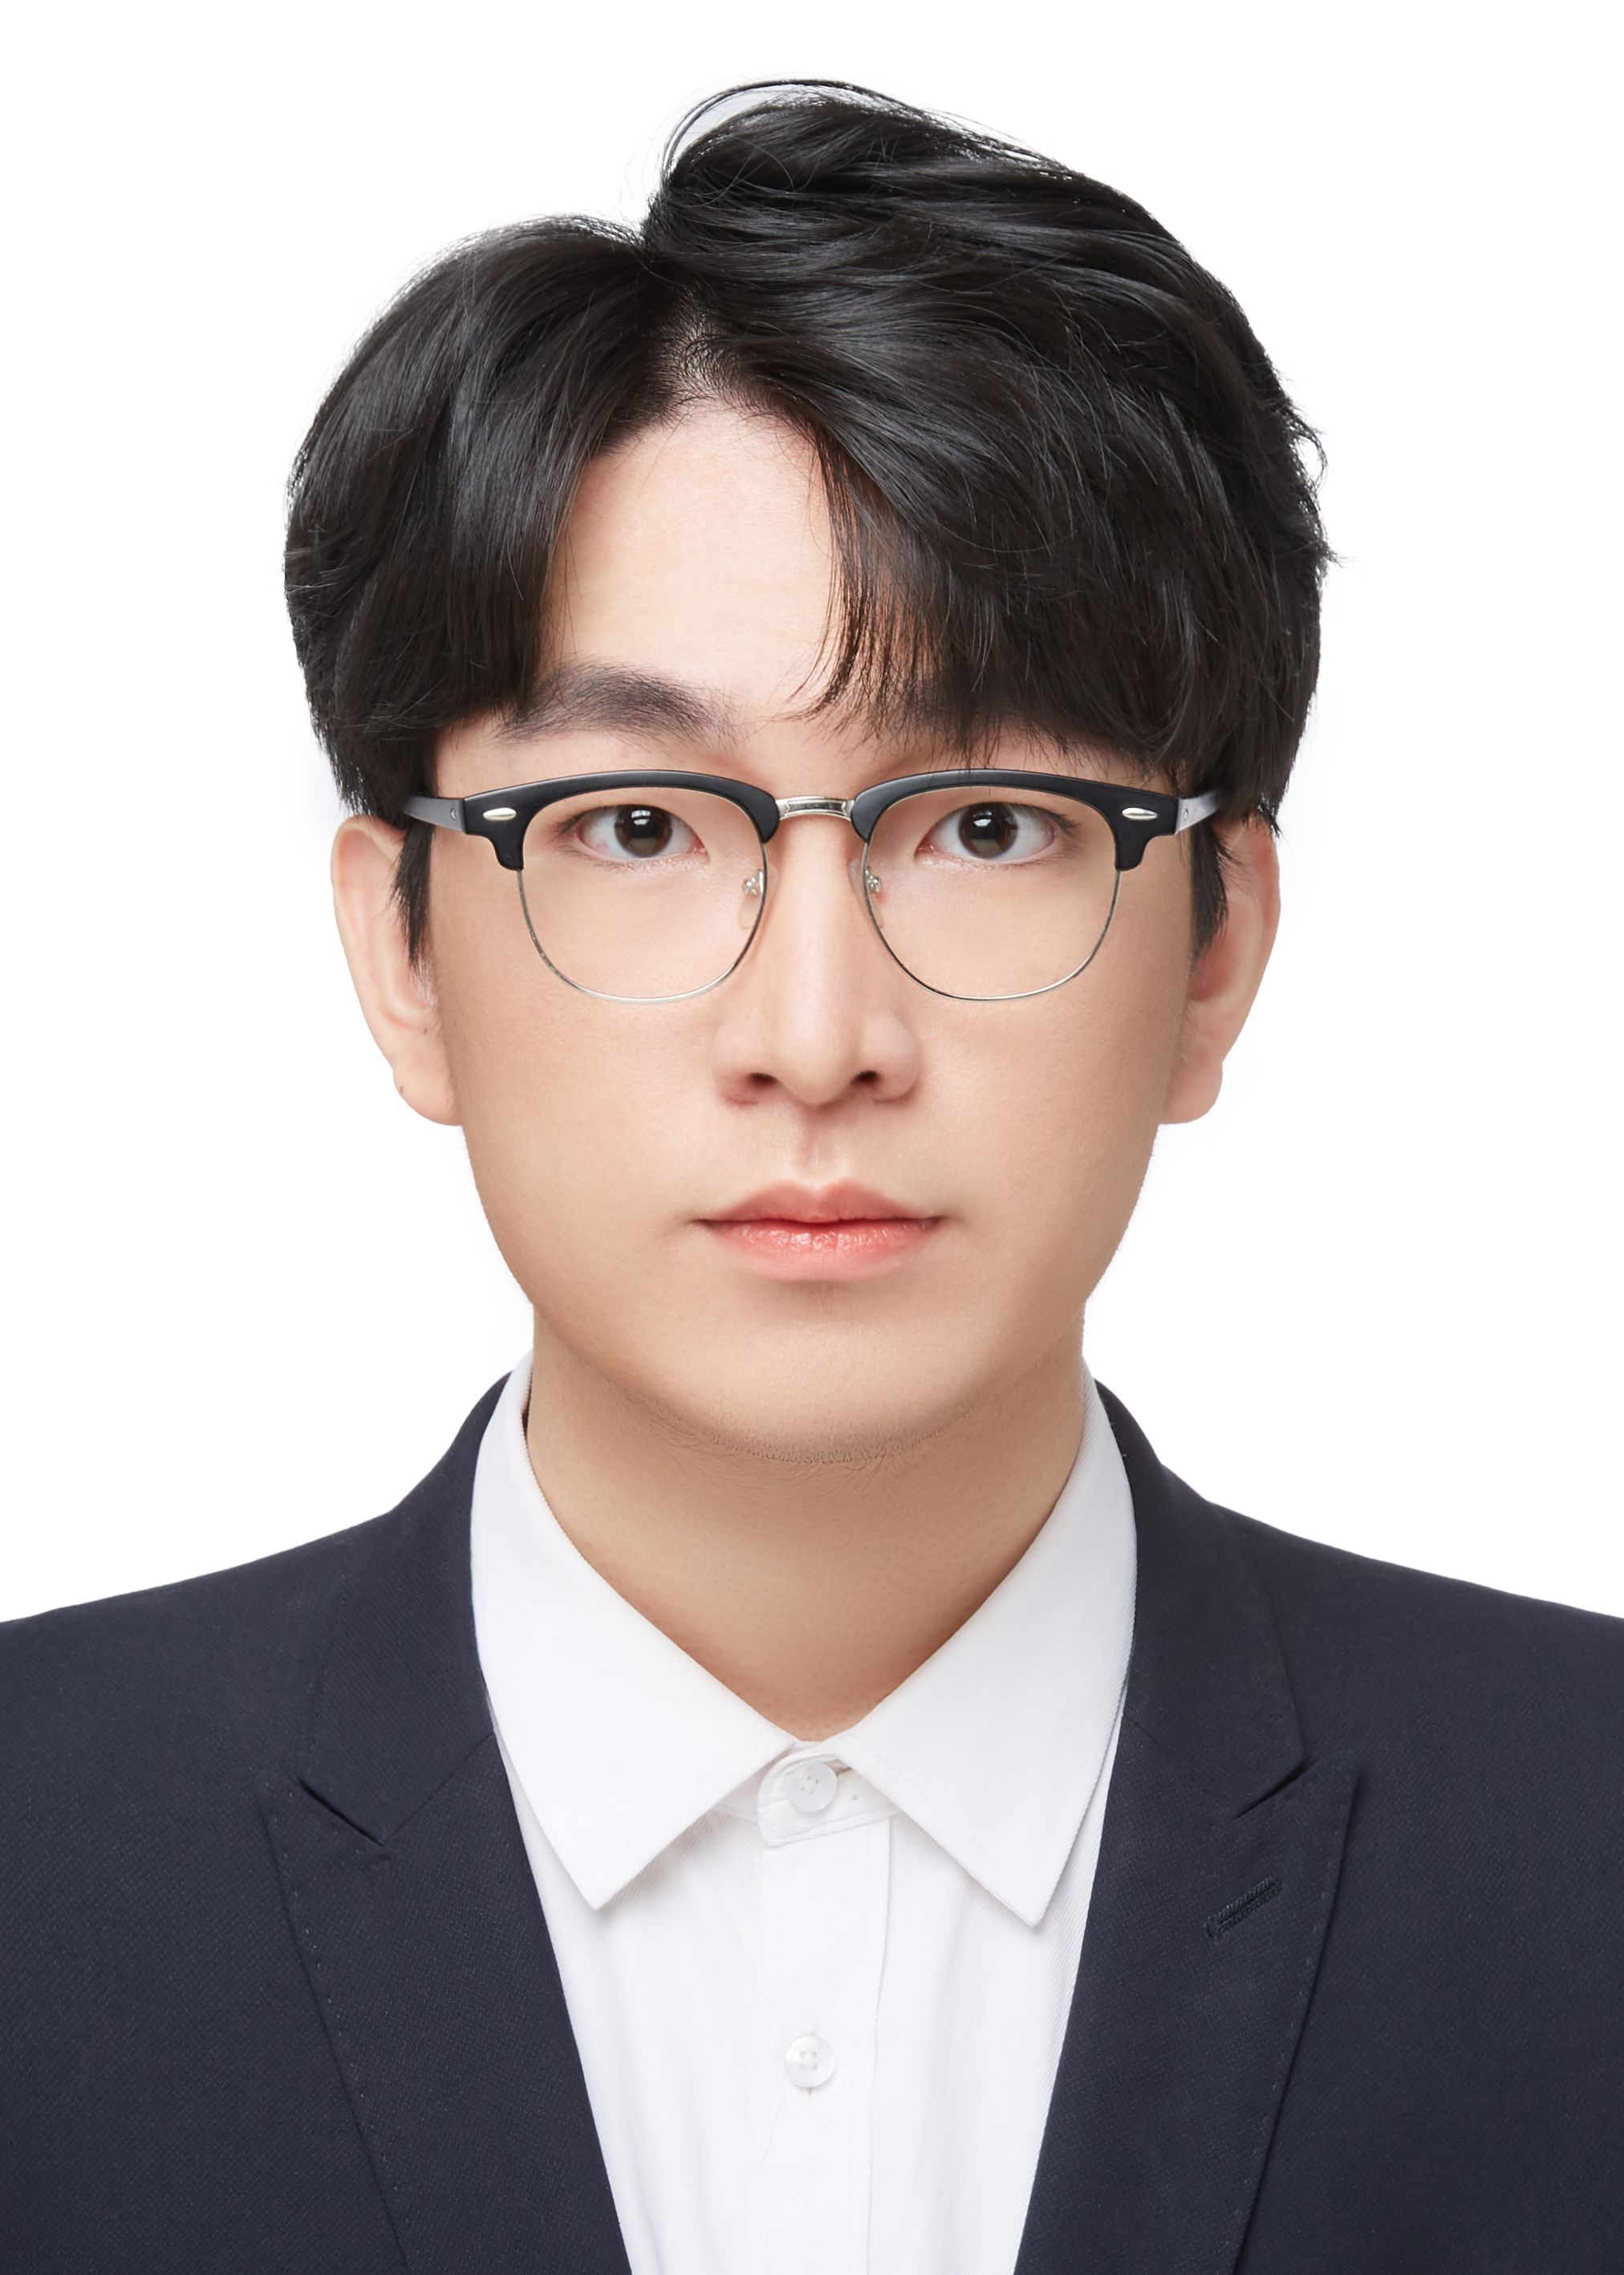
\includegraphics[width=3cm]{LIHONGYANG.jpg}};
\end{tikzpicture}

\ResumeTitle

\vspace{0.5cm}
\section{\textbf{教育背景}}
\ResumeItem
[浙江大学|硕士研究生]
{浙江大学}
[\textnormal{计算生物学,工程师学院|} 工学硕士]
[2023.08—2026.03]
\begin{itemize}
    \item 主要研究方向为\textbf{数据挖掘与医学人工智能},在深度学习、自然语言处理和大数据技术等方面有一定的研究经验.
\end{itemize}

\ResumeItem
[哈尔滨工业大学|本科生]
{哈尔滨工业大学}
[\textnormal{自动化,控制科学与工程系|} 工学学士]
[2019.08—2023.06]
\begin{itemize}
    \item 获中国大学生数学建模竞赛(CUMCM)国家级二等奖,哈工大英才学院荣誉学士学位,英才学院一等奖学金.
\end{itemize}


\section[技术能力]{\textbf{技术能力}}
\begin{itemize}
\item \textbf{主修课程}:离散数学(99),计算机视觉应用(93),系统工程(96),工科数学分析(91),数学物理方程(88).
  \item \textbf{语言}: 在研究工作中有多种语言的应用经验.常用C/C++,Python,R; 熟悉 Java, Scala, JavaScript.
  \item \textbf{工作流}: Linux, Shell, LaTeX, Git, Matlab, Markdown.
  \item \textbf{其他}: \textbf{CET-6:555分},有一定的数学和计算机科学基础,熟悉相关领域的底层理论.
\end{itemize}

\section{\textbf{工作经历}}

\ResumeItem{浙江同花顺智能科技有限公司}
[大数据开发实习生]
[2022.06—2022.09] 

\begin{itemize}
  \item \textbf{结合AI算法和金融理论,对金融市场相关的数据进行研究和建模},基于海量的金融数据,开发在\textbf{特征提取、价格预测、组合优化}等不同的应用场景的智能算法.开发算法优化投资组合的配置,最大化收益并控制风险.
\end{itemize}
\ResumeItem{拾贝投资有限公司}
[量化策略研究员实习生(深度学习方向)]
[2024.09—2024.12] 

\begin{itemize}
  \item \textbf{利用深度学习技术构建复杂预测模型,分析不同因子结合不同学习算法对股票收益的预测效果,进行模型输入端因子的特征工程研究},并结合传统金融模型捕捉市场中的非线性关系。训练在不同方案下应用的交易模型,评估投资组合的潜在风险敞口,并设计智能对冲方案。
\end{itemize}


\section{\textbf{项目经历}}
\ResumeItem{基于OpenCV和偏振光导航技术的计算机视觉系统设计}
[ 哈尔滨工业大学控制与仿真中心]
\begin{itemize}
  \item 设计了一种利用自然太阳光偏振信息进行坐标计算的小型化系统设计方案
  \item 采用CCD工业级相机与卫星感光元件协同设计和自研图像解析算法程序
\end{itemize}

\ResumeItem{基于深度学习的PCR引物设计}
[ 哈尔滨工业大学智能控制研究所]
\begin{itemize}
  \item 扩展了已有的单重PCR(聚合酶链式反应)引物设计算法,建立了多重PCR引物设计问题的数学模型
  \item 采用自然语言处理技术、深度学习方法和压缩感知理论等建立了多重PCR引物设计算法的理论基础
  \item 完成了多重PCR技术引物设计的语言模型和图模型算法设计
\end{itemize}


\ResumeItem{基于模态逻辑的思维图谱推理系统设计}
[ 浙江大学基础医学院生物信息学系]
\begin{itemize}
  \item 在模态逻辑理论的基础上,提出一种以完备的数据结构形式表述自然语言中知识和逻辑体系的方法
  \item 以可解释的人工标注为媒介,通过用户操作和自动校正实现了系统知识理解正确性与可靠性的自动确认
  \item 实现了给定框架下全新知识的生成和对用户所提出问题的自动判断
\end{itemize}



\section{\textbf{个人总结}}

\begin{itemize}
  \item 乐观开朗,在校成绩优异,具有良好的沟通能力和团队合作精神.
  \item 可以熟练使用英语进行工作交流,在科研工作中主要使用英文作为工作语言,平时有阅读英文书籍和视听练习的习惯.
  \item 有丰富的代码编写和维护经验,善于技术写作,持续关注互联网技术发展。
\end{itemize}


\end{document}
